% Please make sure you insert your
% data according to the instructions in PoSauthmanual.pdf
\documentclass[a4paper,11pt]{article}
\usepackage{pos}

\title{Recent results in Higgs physics}
%% \ShortTitle{Short Title for header}

\author*[a]{Emanuele Di Marco}
\onbehalf{on behalf of the CMS collaboration}

\affiliation[a]{Istituto Nazionale di Fisica Nucleare (INFN), Sezione di Roma1,\\
  Piazzale Aldo Moro n. 2, 00185, Rome, Italy}

\emailAdd{emanuele.dimarco@roma1.infn.it}

\abstract{This document summarizes recent results from ATLAS and CMS
  collaborations in the measurements of properties and searches of
  Beyond Standard Model effects in Higgs boson physics, using data
  from LHC Runs 2 and 3. The focus is on recent results of
  differential cross section measurements, with their interpretation
  in EFTs, as well analyses probing the CP structure of the couplings
  with vector bosons and tau leptons. Updated measurements of rare
  processes, as $\textrm{H} \to\mu\mu$ or
  $\textrm{H}\to\textrm{Z}\gamma$ are presented, as well as results on
  double or triple Higgs boson productions.  }

\FullConference{The European Physical Society Conference on High Energy Physics (EPS-HEP2025)\\
7-11 July 2025\\
Marseille, France\\}

%% \tableofcontents

\begin{document}
\maketitle


\section{Introduction}

In the ten years since the discovery of the Higgs boson by the
ATLAS~\cite{ATLAS:2008xda,ATLAS:2012yve} and
CMS~\cite{CMS:2008xjf,CMS:2012qbp,CMS:2013btf} Collaborations, much
has been learned about this particle. Most of the major production
modes and decay channels have been observed, and with the data
collected during Run 2 (2015–2018) and Run 3 (2022-2024) of the LHC it
is possible to probe the cross sections and properties with increasing
precision.  Cross section measurements can be made with different
levels of granularity. Inclusive signal strength or cross section
measurements are performed when the analyzed data set is small. With
more data it is possible to measure simplified template cross sections
(STXS), in which the production modes are divided into regions as a
function of one or more kinematical variables. Their results can be
interpreted in terms of couplings to Standard Model particles, as well
as in Effective Field Theories. The larger datasets allow access to
rare decay modes of the Higgs boson, as the ones into second
generation fermions, or to $\textrm{Z}\gamma$.

\section{Higgs Boson Production and Decay Measurements}

Measurements of Higgs boson production and decay rates were performed
by the ATLAS and CMS experiments using up to $140~\text{fb}^{-1}$ of
proton--proton collisions collected at $\sqrt{s} = 13~\text{TeV}$
during Run~2 of the LHC. The results combine the most recent analyses
available for each production and decay process.

Combined measurements of Higgs boson production and
decay rates, as well as STXS. In
the STXS framework, the phase space of different Higgs
production modes is divided into non-overlapping regions (\emph{STXS
bins}) defined by event kinematics, providing finer information beyond
inclusive rate measurements. Results are reported at two levels of
granularity: \textbf{stage~0}, corresponding to major production
modes, and \textbf{stage~1.2}, the latest definition used here, which
further subdivides bins by kinematic properties~\cite{stxs}. The
measurements are also interpreted within the coupling
modifier and \textsc{SMEFT}~\cite{smeft} frameworks.

The combination includes the decay channels $H \to \gamma\gamma$, $H
\to ZZ \to 4\ell$, $H \to WW \to \ell\nu\ell\nu$, $H \to \tau\tau$, $H
\to bb$, $H \to \mu\mu$, and $H \to Z\gamma$, along with searches for
$H \to \text{inv}$, constraining the branching fraction to
beyond-the-Standard-Model final states. Each channel targets multiple
production mechanisms: gluon--gluon fusion (ggH), vector boson fusion
(VBF), associated production with a vector boson (VH, $V = W$ or $Z$),
top-quark pair production (ttH), and single-top production (tH). ZH
production includes both $qqZH$ and $ggZH$ components, while tH
includes $tHW$ and $tHq$ modes. Although $bbH$ production is not
directly measured, its small contribution is included in the signal
model. Additionally, an off-shell Higgs analysis constrains the total
Higgs decay width directly from data.

The overall Higgs boson signal strength ($\mu$), relative to the
Standard Model (SM) expectation, is found to be consistent with the SM
prediction, with an uncertainty between 5 and 6\%.  The dominant
contribution to this uncertainty arises from theoretical uncertainties
on the SM prediction, rather than from experimental or statistical
sources.

STXS for Higgs boson production processes are found to be consistent
with the SM within relative uncertainties of 6\% to 18\%. Compared to
previous results with smaller number of analyses included, or smaller data set, the uncertainties in the production rates for $WH$,
$ZH$, and $t\bar{t}H + tH$ processes are reduced by approximately
30\%, 20\%, and 40\%, respectively.

In the most recent combination performed by ATLAS, branching fractions for the main Higgs boson decay modes,
$
H \to \gamma\gamma, \quad
H \to ZZ^* \to 4\ell, \quad
H \to WW^* \to \ell\nu\ell\nu, \quad
H \to b\bar{b}, \quad
H \to \tau\tau,
$
are measured with relative uncertainties between 8\% and 13\%, all consistent with SM expectations. 
The uncertainties in the $H \to b\bar{b}$ and $H \to WW^*$ branching ratios are reduced by about 20\%, 
and the uncertainty in the $H \to \tau\tau$ branching ratio by about 10\%, relative to Ref.~\cite{atlas-comb}. 
Additionally, products of cross sections and branching ratios are reported for 29 combinations of 
production and decay channels.

Interpretations in terms of Higgs boson coupling modifiers are also
presented. Assuming only SM contributions to loop processes and to
Higgs boson processes not directly probed in the analyses, the
couplings to $W$, $Z$, $t$, $b$, and $\tau$ are measured with
uncertainties between 5\% and 12\%, representing improvements of
10\%--20\% compared to previous measurements. The coupling to the muon
is measured with an uncertainty of about 25\%, and the coupling to the
charm quark with an asymmetric uncertainty of $^{+1.6}_{-3.8}$,
corresponding to roughly a twofold improvement over
Ref.~\cite{atlas-comb}.

The measurement of the production cross-sections for the main Higgs
boson production processes, assuming s the SM Higgs boson branching
fractions, is reported in Fig.~\ref{fig:stxs} (left). The most
granular fit performed by CMS is done by introducing a separate
parameter of interest for each branching ratio, for each STXS bin,
resulting in 97 POIs~\cite{cms-comb}, and it is shown in
Fig.~\ref{fig:stxs}.

\begin{figure}[!tbp]
\centering
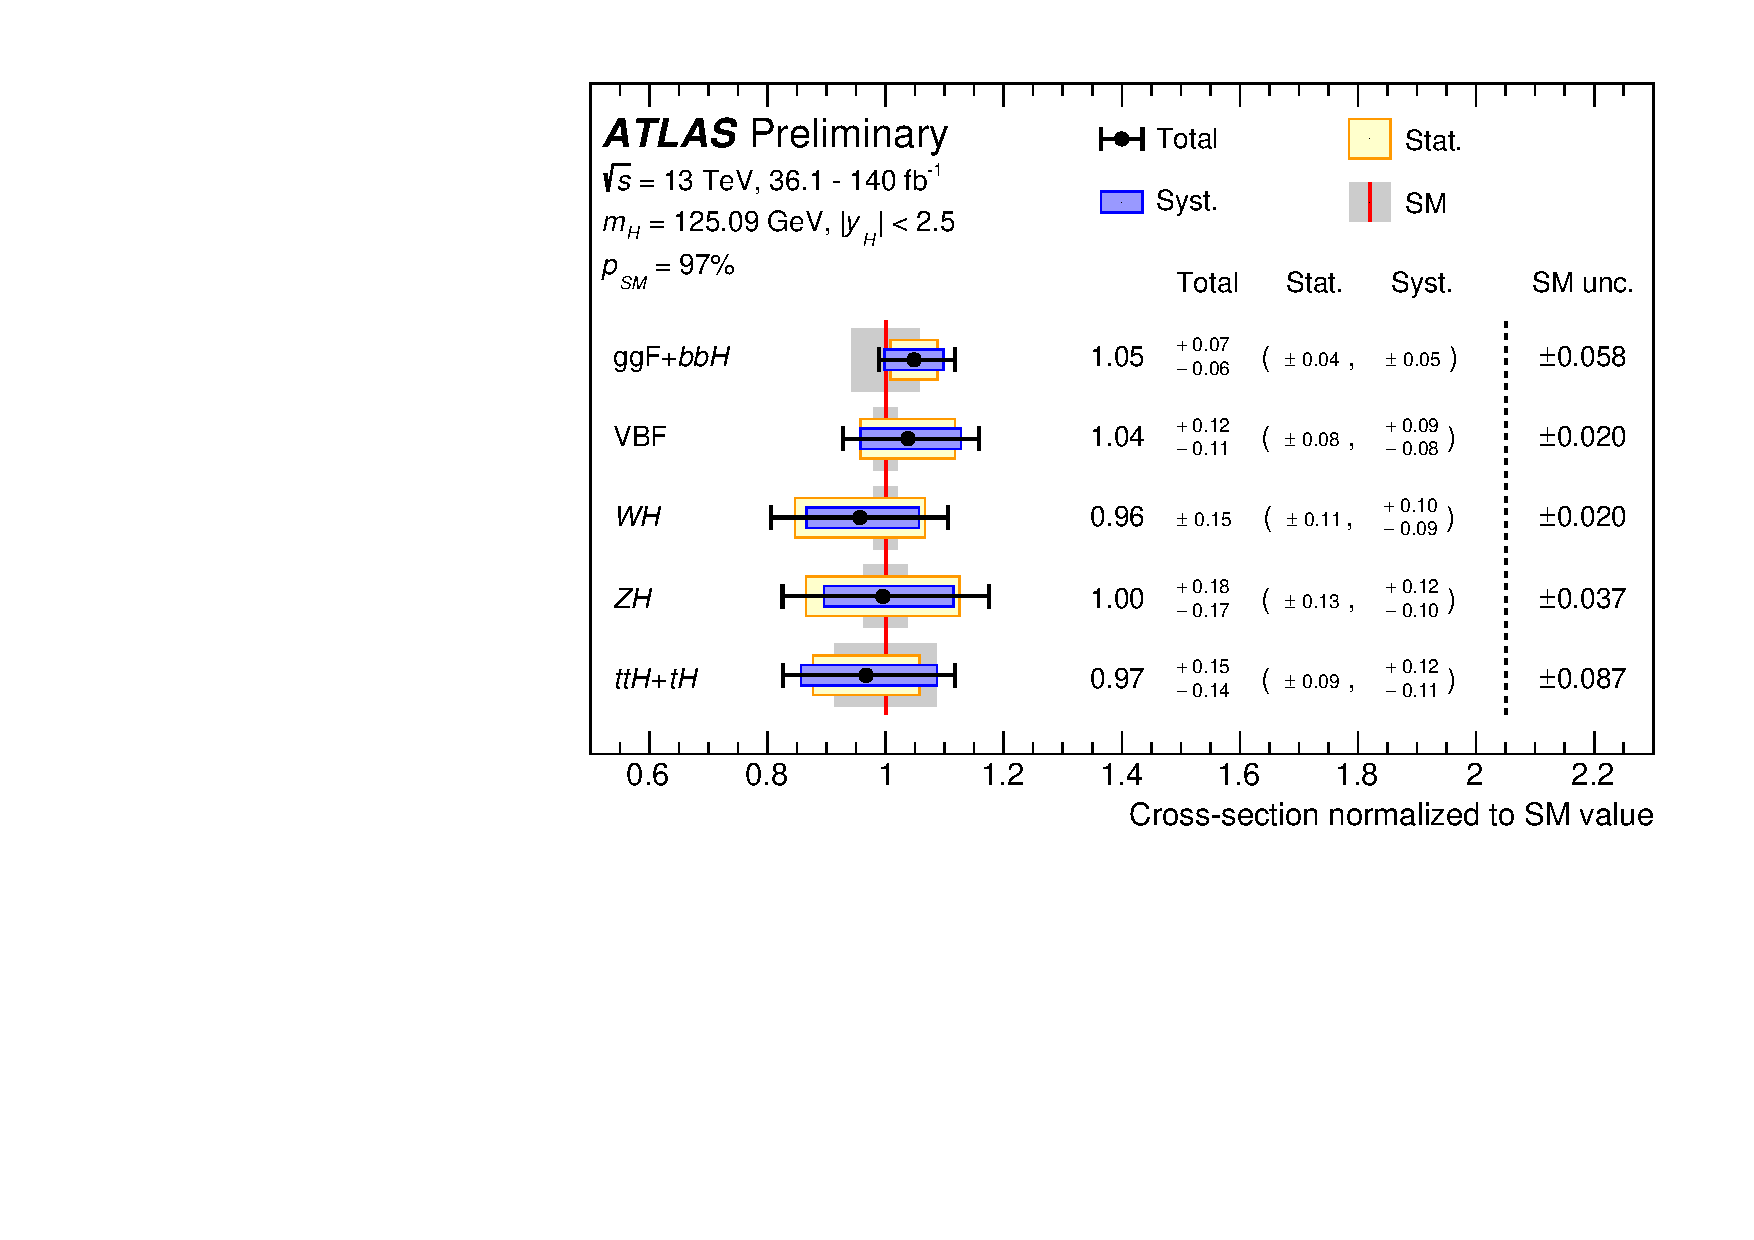
\includegraphics[width=0.4\textwidth]{stxs-atlas-xsecs}
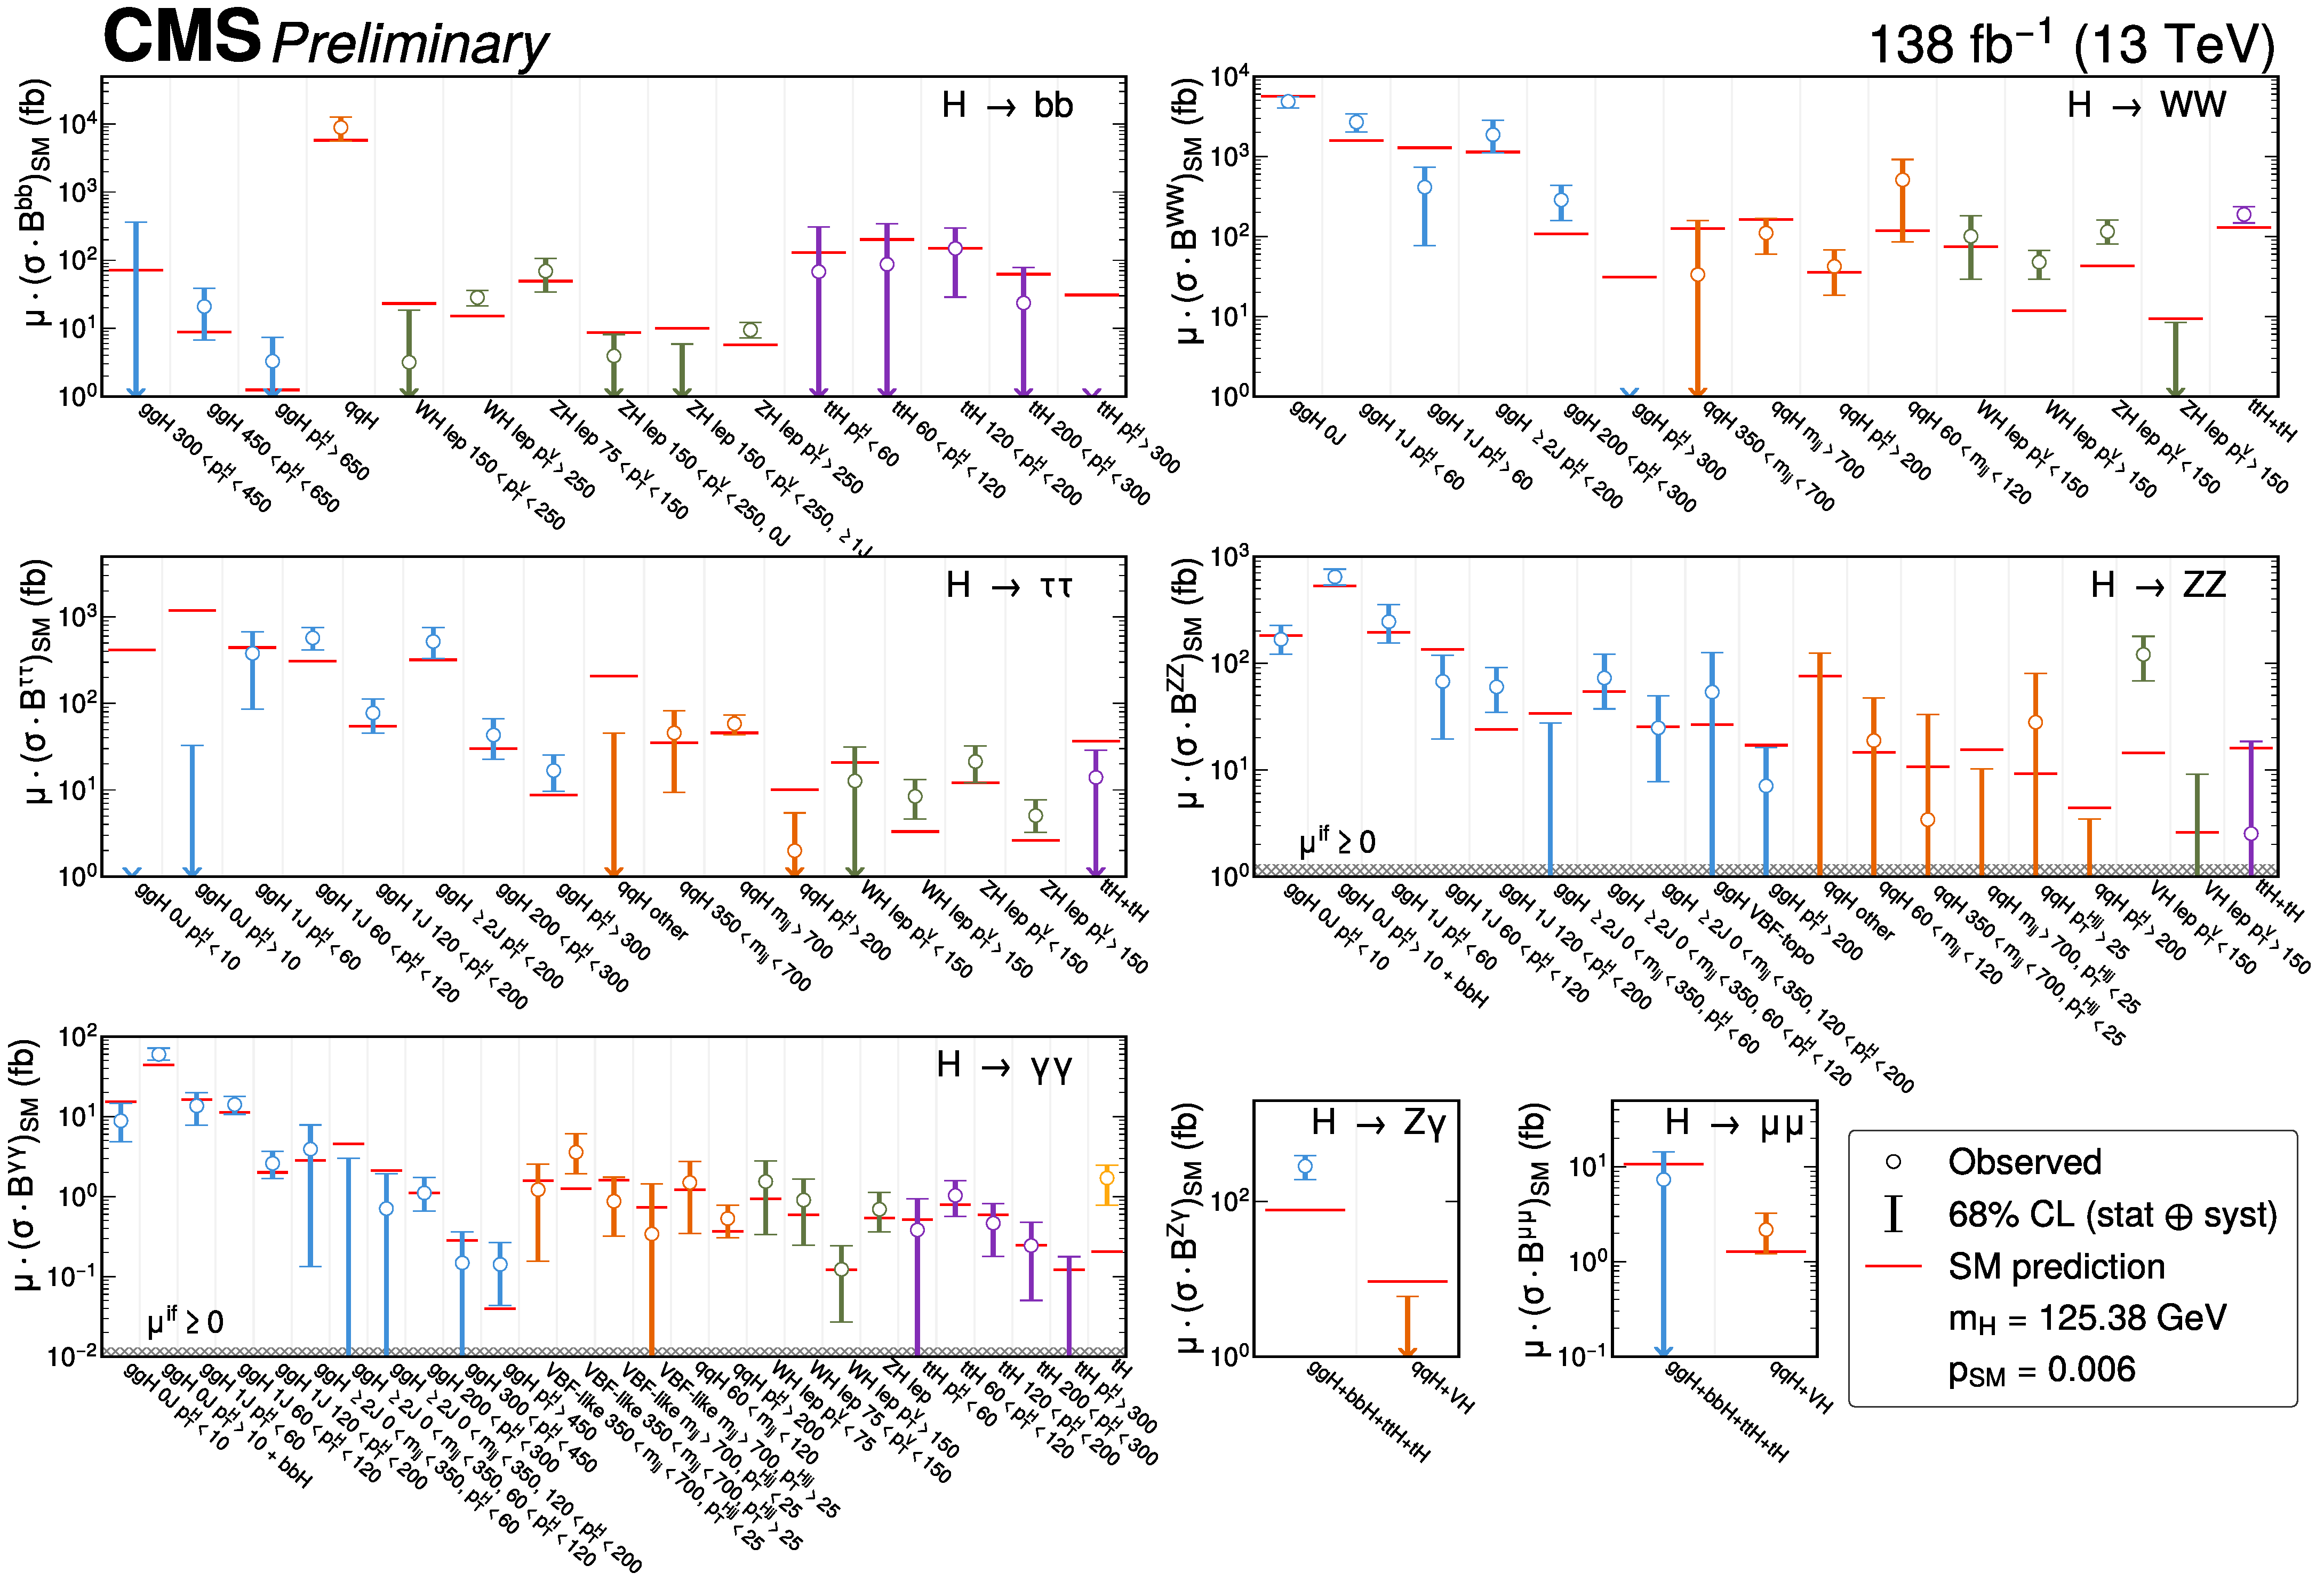
\includegraphics[width=0.4\textwidth]{stxs-cms-xsecs}
\caption
{Observed cross sections values for the main Higgs bosonproduction
  modes, relative to their SM predictions, as measured in the most
  recent ATLAS combination~\cite{atlas-comb} (left). Best fit values
  (white circles) and 68\% CL intervals (coloured lines) for the cross
  section times branching fraction fit in the most recent CMS
  combination~\cite{cms-comb}.
\label{fig:stxs}
}
\end{figure}

All measurements are found to be in excellent agreement with Standard Model predictions.





\bibliographystyle{JHEP}
\bibliography{dimarco}

\end{document}


